\subsubsection{ROC-AUC Analysis}

The ROC-AUC analysis evaluates the ability of the final XGBoost model to distinguish between favorable and risky credit applications across all possible decision thresholds. The ROC curve plots the true positive rate against the false positive rate, while the diagonal line represents the behavior of a random classifier.

\begin{figure}[htbp]
\centering
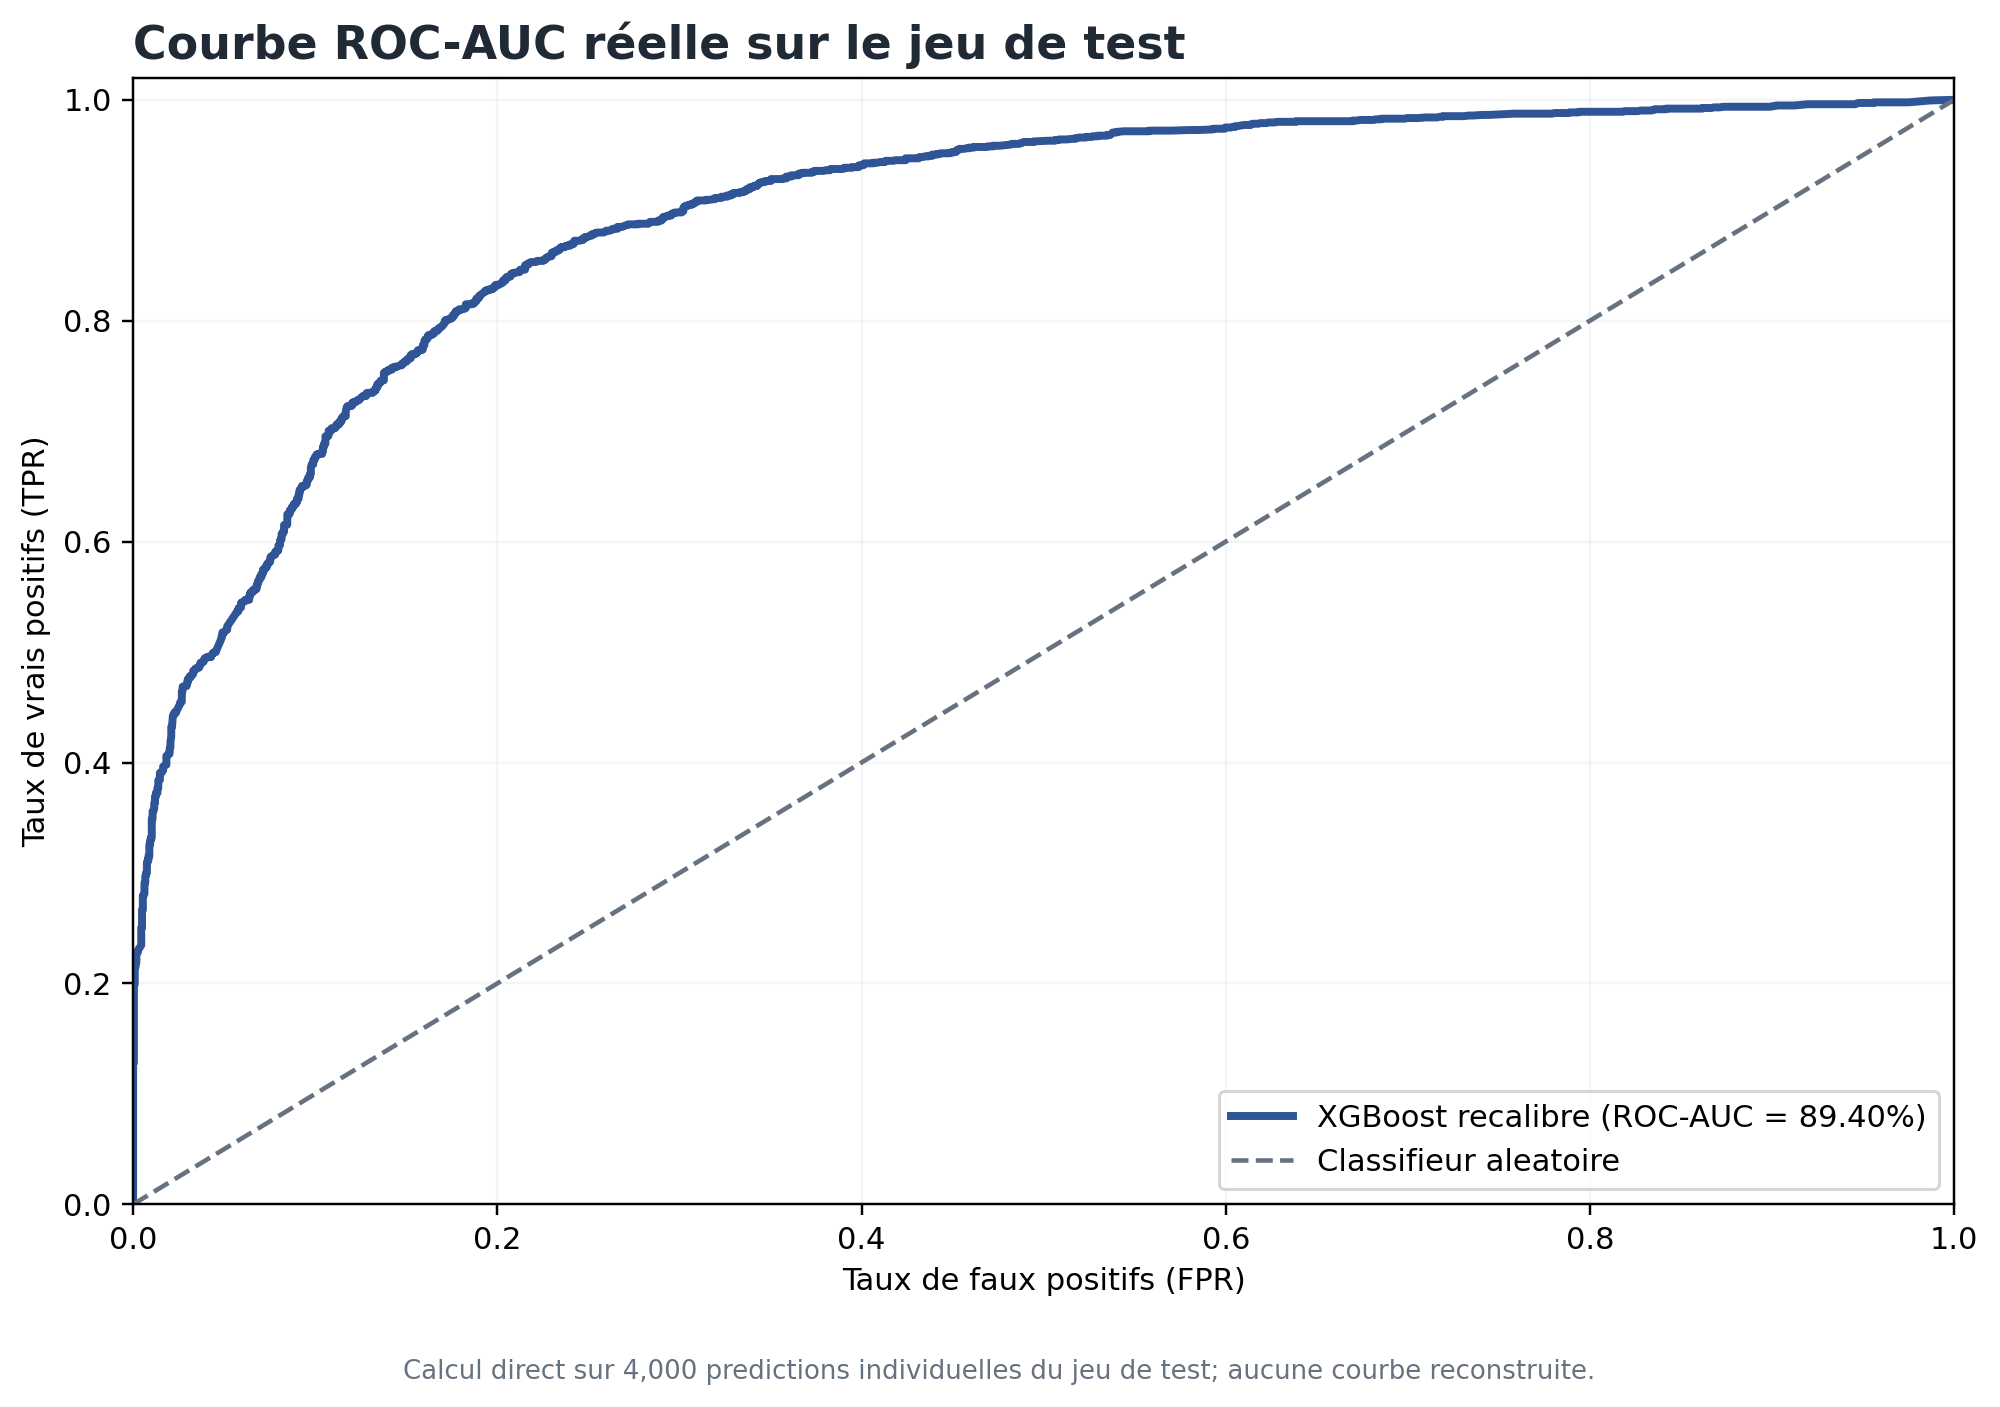
\includegraphics[width=0.85\textwidth]{../img/53_xgboost_roc_curve.png}
\caption{ROC-AUC analysis of the final XGBoost model}
\label{fig:xgboost_roc_auc_analysis}
\end{figure}

The governed XGBoost model achieves a test ROC-AUC of 89.17\%, calculated directly from 4,000 individual out-of-sample predictions. The curve is not reconstructed from an aggregated reporting value and the AUC is not capped. This result uses a conservative set of 18 application variables that excludes the main proxies for the synthetic decision rule.

The corresponding Gini coefficient is 78.35\%, calculated as:

\[
Gini = 2 \times AUC - 1
\]

This value confirms the model's ability to rank applicants according to their level of credit risk. A higher Gini coefficient indicates better separation between low-risk and high-risk profiles, which is important in credit scoring because the model is not only expected to classify applications, but also to prioritize applicants by risk level.

However, ROC-AUC does not directly determine the optimal operational threshold. In credit risk assessment, the final threshold must be selected according to business priorities. A lower threshold increases the detection of risky applications but may reject more favorable clients, while a higher threshold reduces false alerts but may miss some risky clients.

Since the dataset used in this project is synthetic, the ROC-AUC result should be interpreted as a methodological validation of the machine learning pipeline and not as evidence of production-level banking performance. A real banking deployment would require validation on historical, anonymized, and representative banking data.
